\documentclass[conf]{new-aiaa}
%\documentclass[journal]{new-aiaa} for journal papers
\usepackage[utf8]{inputenc}

\usepackage{graphicx}
\usepackage{amsmath}
\usepackage{commath}
\usepackage[version=4]{mhchem}
\usepackage{siunitx}
\usepackage{longtable,tabularx}
\usepackage{float}
\usepackage{listings}
\usepackage{pdfpages}
\usepackage{color} %red, green, blue, yellow, cyan, magenta, black, white
\definecolor{mygreen}{RGB}{28,172,0} % color values Red, Green, Blue
\definecolor{mylilas}{RGB}{170,55,241}
\setlength\LTleft{0pt} 

\lstset{language=Matlab,%
	basicstyle=\footnotesize,
	breaklines=true,%
	morekeywords={matlab2tikz},
	keywordstyle=\color{blue},%
	morekeywords=[2]{1}, keywordstyle=[2]{\color{black}},
	identifierstyle=\color{black},%
	stringstyle=\color{mylilas},
	commentstyle=\color{mygreen},%
	showstringspaces=false,%without this there will be a symbol in the places where there is a space
	numbers=left,%
	numberstyle={\tiny \color{black}},% size of the numbers
	numbersep=9pt, % this defines how far the numbers are from the text
	emph=[1]{for,end,break},emphstyle=[1]\color{red}, %some words to emphasise
	%emph=[2]{word1,word2}, emphstyle=[2]{style},    
}

% ================================================================ % 
\title{ASE 389P.4 Methods of Orbit Determination \\ Homework 2: Orbit Propagation with Perturbations}

\author{Junette Hsin}
\affil{Masters Student, Aerospace Engineering and Engineering Mechanics, University of Texas, Austin, TX 78712}

\begin{document}

\maketitle

\begin{abstract}
New force models have been added to the orbit propagator created in Homework 1. The effects that these new forces have on the Keplerian orbit elements and the
total specific energy were analyzed.

\end{abstract}


% ================================================================ % 
\section*{Problem 1}

 % \subsubsection*{Statement} 
\begin{center}
\fbox{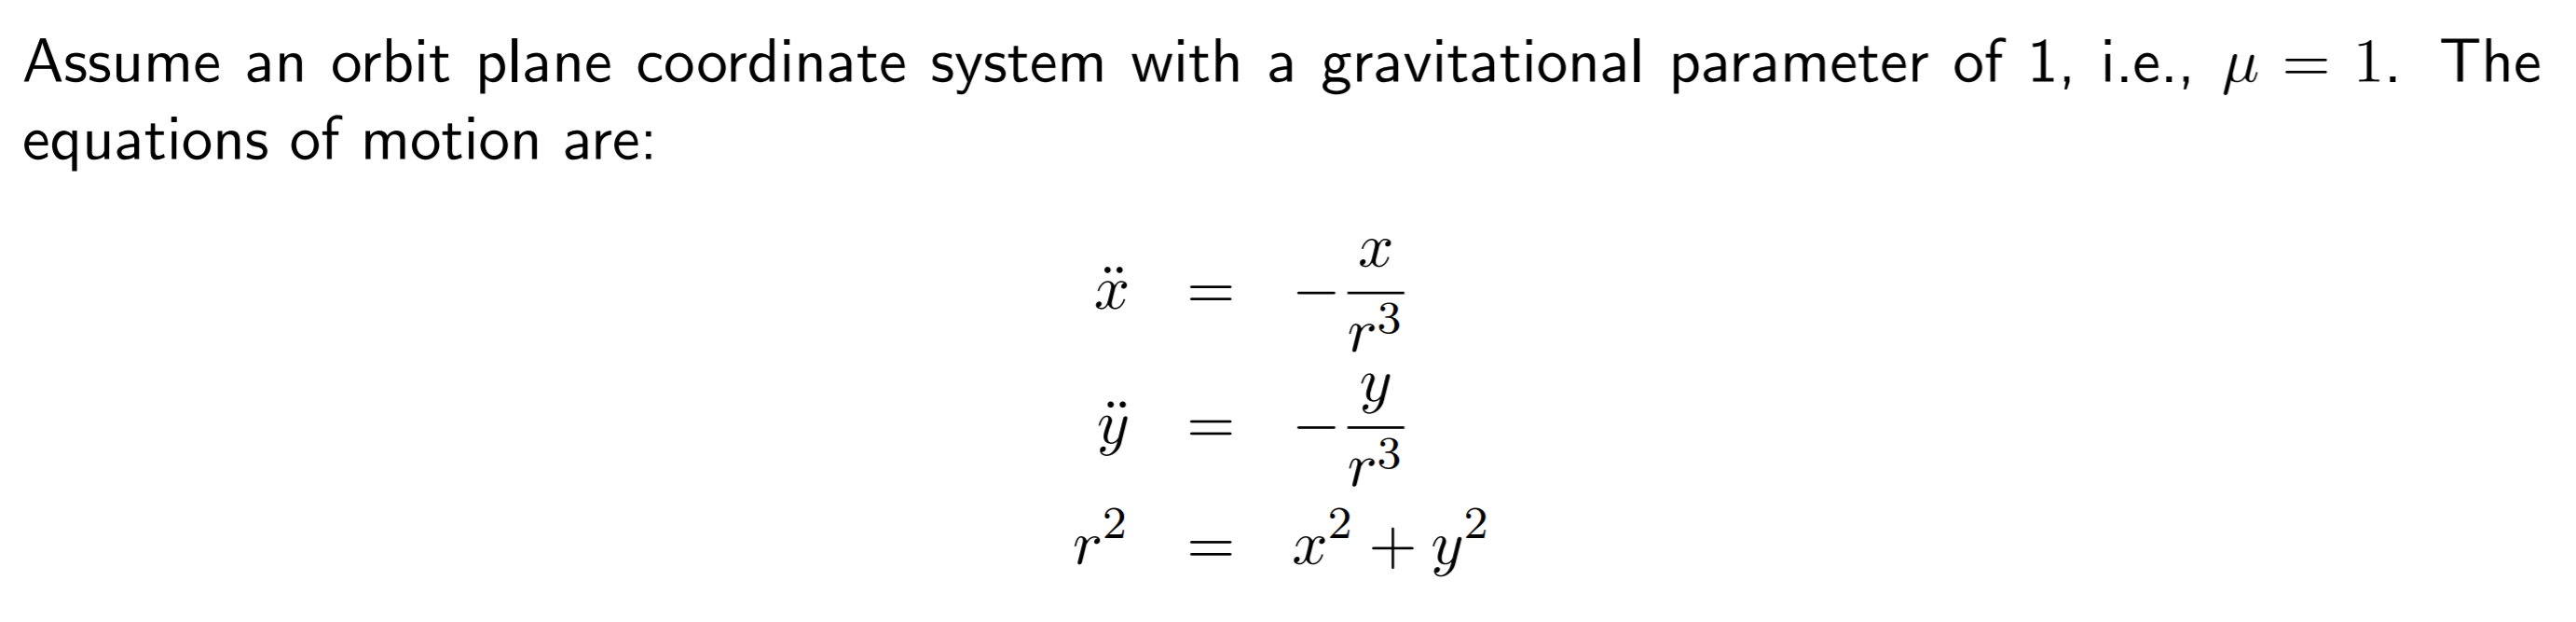
\includegraphics[width=0.9\textwidth]{prob_1.png}} \\
\end{center}

% ---------------------------------------------------------------- % 
\subsubsection*{Solution} 

%The algorithms to convert orbital elements to Cartesian and back were taken from References \cite{bate_astrodynamics} and \cite{jah_mod3}. First, the specific angular momentum vector, $h$, and perpendicular node vector (to the plane of the orbit), $n$, were calculated. Inclination, eccentricity, and the rest of the orbital elements followed while checking for equatorial orbits, NaNs, and quadrants of angles. Given the spacecraft position and velocity vectors from the problem statement, the Keplerian elements are: 
%
%\begin{equation}
%\begin{aligned}
%a = &~ 7.712184983762814e+03 \\ 
%e = &~ 0.447229247404423 \\ 
%i = &~ 1.570796326794897 \\ 
%\omega = &~ 3.139593866862924 \\ 
%\Omega = &~ 3.926990816987241 \\ 
%\nu = &~ 2.032461649676350  
%\end{aligned}
%\end{equation}
%
%where $a$ is the semi-major axis, $e$ is the eccentricity, $i$ is the orbit inclination, $\omega$ is the argument of perigee, $\Omega$ is the right ascension of the ascending node, and $\nu$ is the true anomaly. 


\newpage
% ================================================================ % 

\subsection*{Problem 1a} 

 % \subsubsection*{Statement} 
\begin{center}
	\fbox{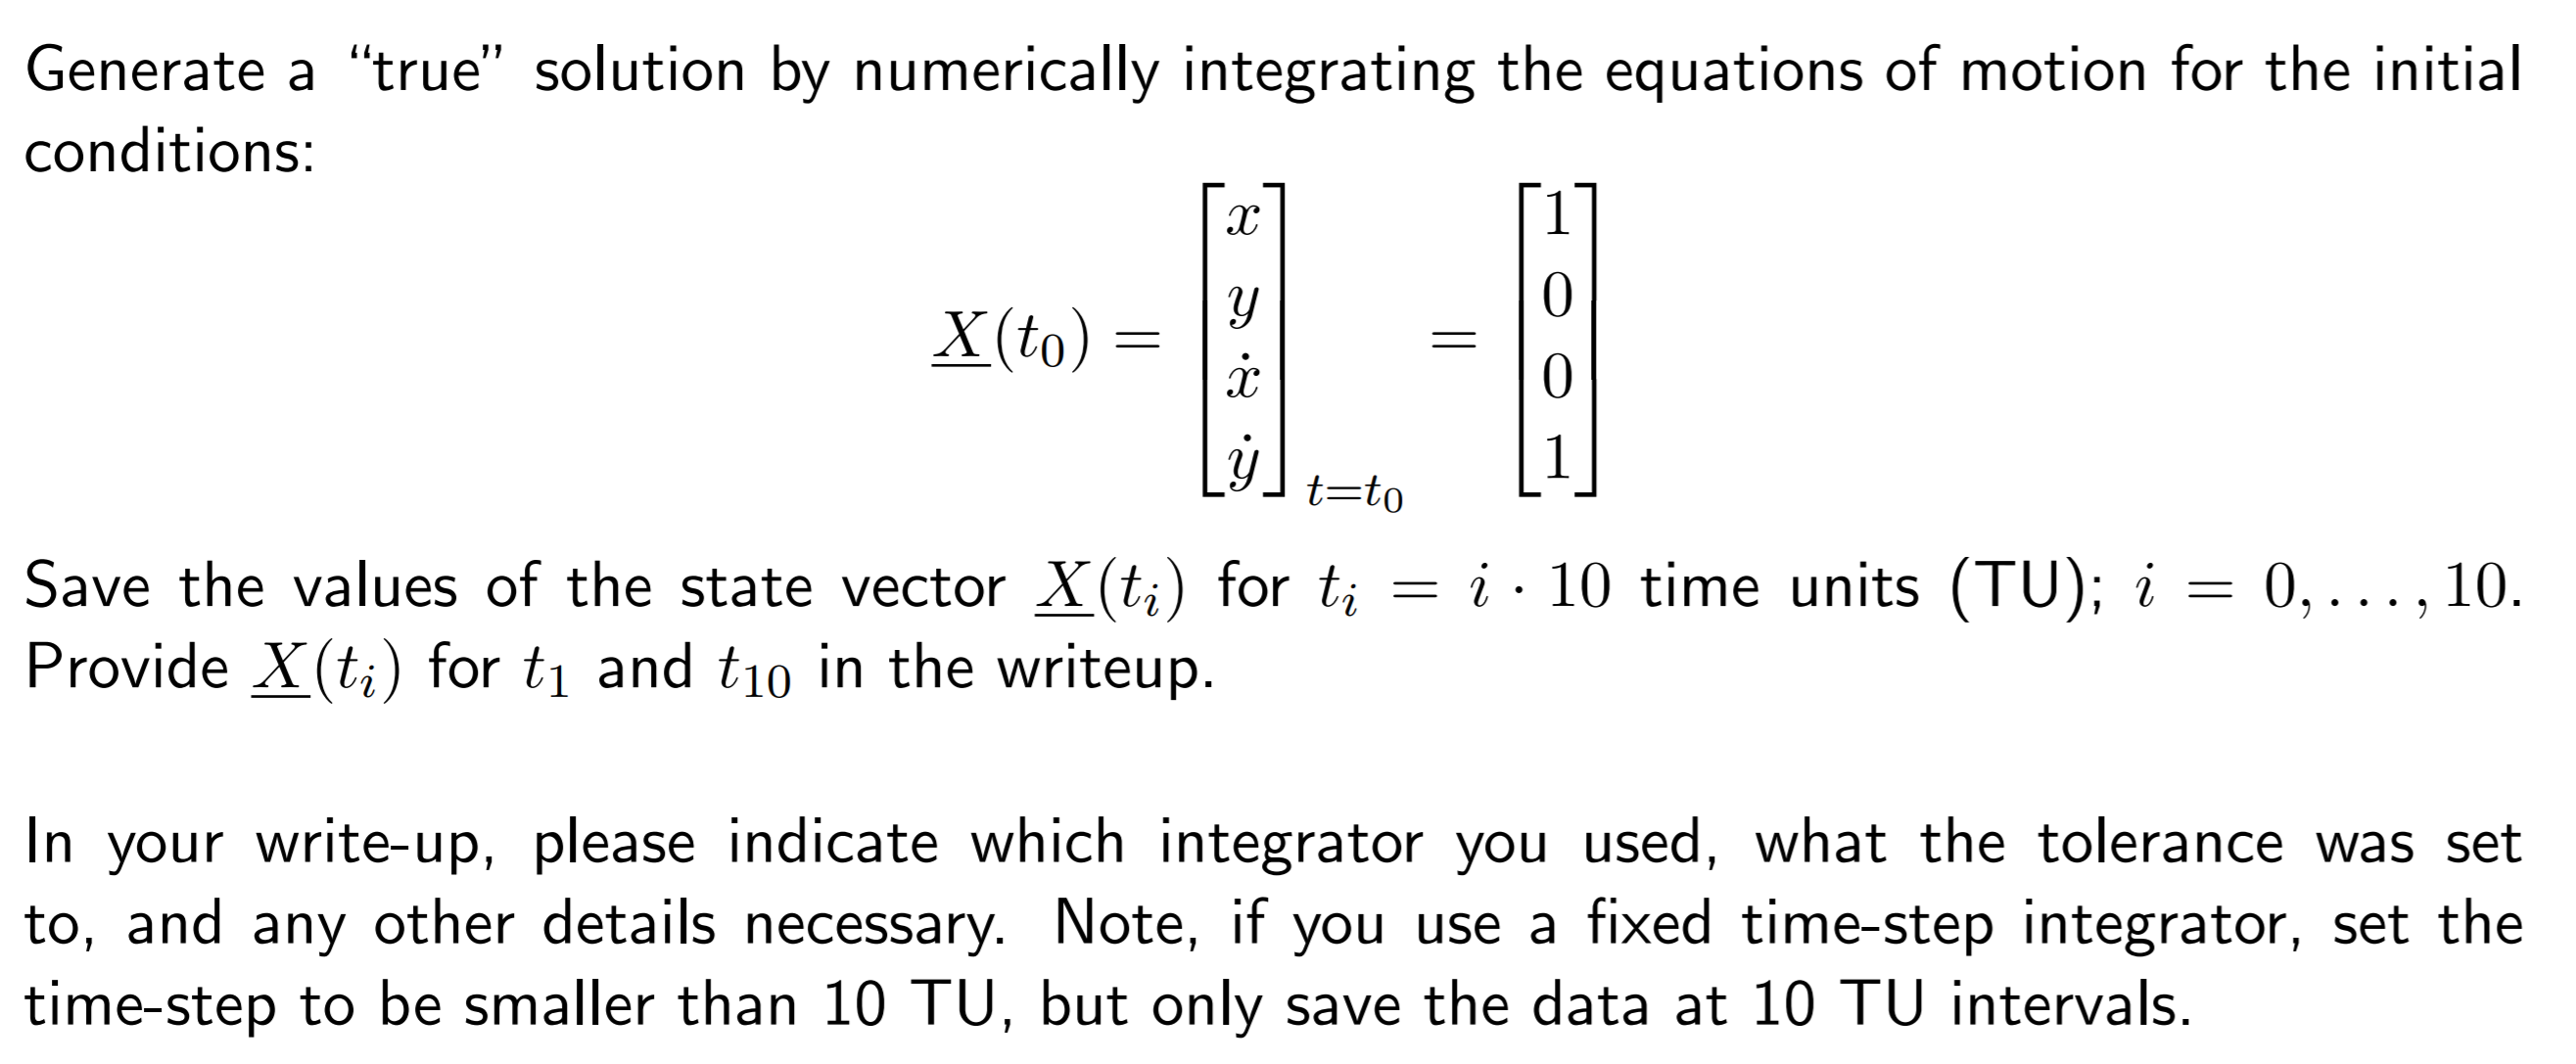
\includegraphics[width=0.9\textwidth]{prob_1a.png}} \\
\end{center}

% ---------------------------------------------------------------- % 

\subsubsection*{Solution} 

%     -(3*J2*RE^2*mu*x*(x^2 + y^2 - 4*z^2))/(2*(x^2 + y^2 + z^2)^(7/2))
%-(3*J2*RE^2*mu*y*(x^2 + y^2 - 4*z^2))/(2*(x^2 + y^2 + z^2)^(7/2))
%-(3*J2*RE^2*mu*z*(3*x^2 + 3*y^2 - 2*z^2))/(2*(x^2 + y^2 + z^2)^(7/2))

The derivation by hand is included in the appendix. The hand-derived and MATLAB results were the same. The final equation for $\partial U / \partial x $ is: 

\begin{equation}
	\partial U / \partial x = -J_2 \mu R_E^2 \Big( \dfrac{3x}{2} \Big) \dfrac{ x^2 + y^2 - 4z^2 }{ (x^2 + y^2 + z^2)^{7/2} }
\end{equation}

The MATLAB code used for the entire homework, including calculating the partial derivatives is included in the Appendix, but the snippet used to solve Problem 1a is shown here: 

\begin{lstlisting}
syms x y z 
global mu RE J2 

% constants 
% mu = 398600.4;      % G * M1 * M2 
% RE = 6378.145;      % Earth radius 
% J2 = 0.00108248;    % J2 

% for symbolic representation 
syms mu RE J2 

% radius 
r = sqrt(x^2 + y^2 + z^2); 

% U point mass 
Up = mu/r; 

% latitude 
phi = asin(z/r); 

% U J2 
UJ2 = -mu/r * J2 * (RE/r)^2 * ( 3/2 * ( sin(phi) )^2 - 1/2 ); 

% gradient 
d_UJ2 = gradient(UJ2, [x y z]); 
d_UJ2 = simplify(d_UJ2); 
\end{lstlisting}

\newpage
% ================================================================ % 

\subsection*{Problem 1b} 

 % \subsubsection*{Statement} 
\begin{center}
	\fbox{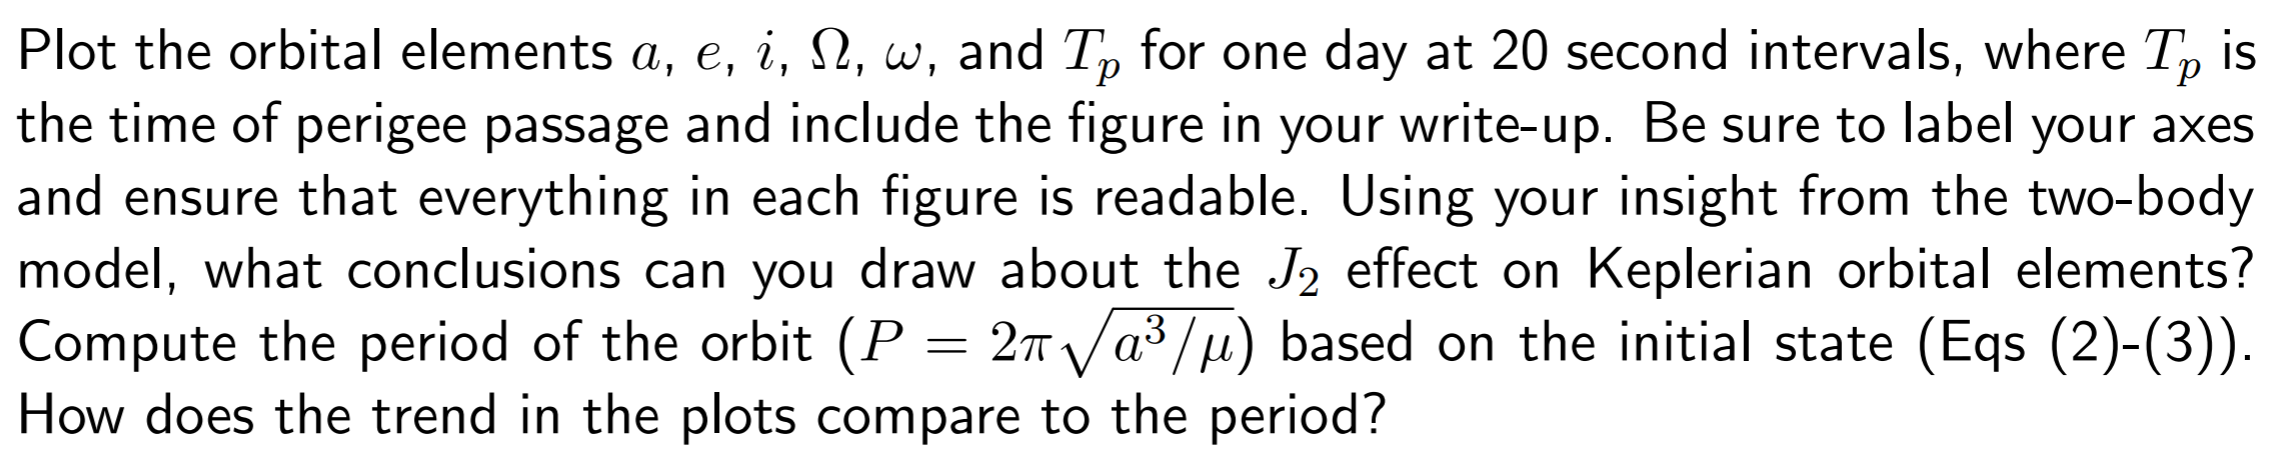
\includegraphics[width=0.9\textwidth]{prob_1b.png}} \\
\end{center}

% ---------------------------------------------------------------- % 

\subsubsection*{Solution} 

Based on the initial state, the period of the orbit is: 

\begin{equation}
	P = 2 \pi \sqrt{ a^3 / \mu } = 6.740270469266463e+03 s 
\end{equation}

\begin{figure}[H]
	\centering
	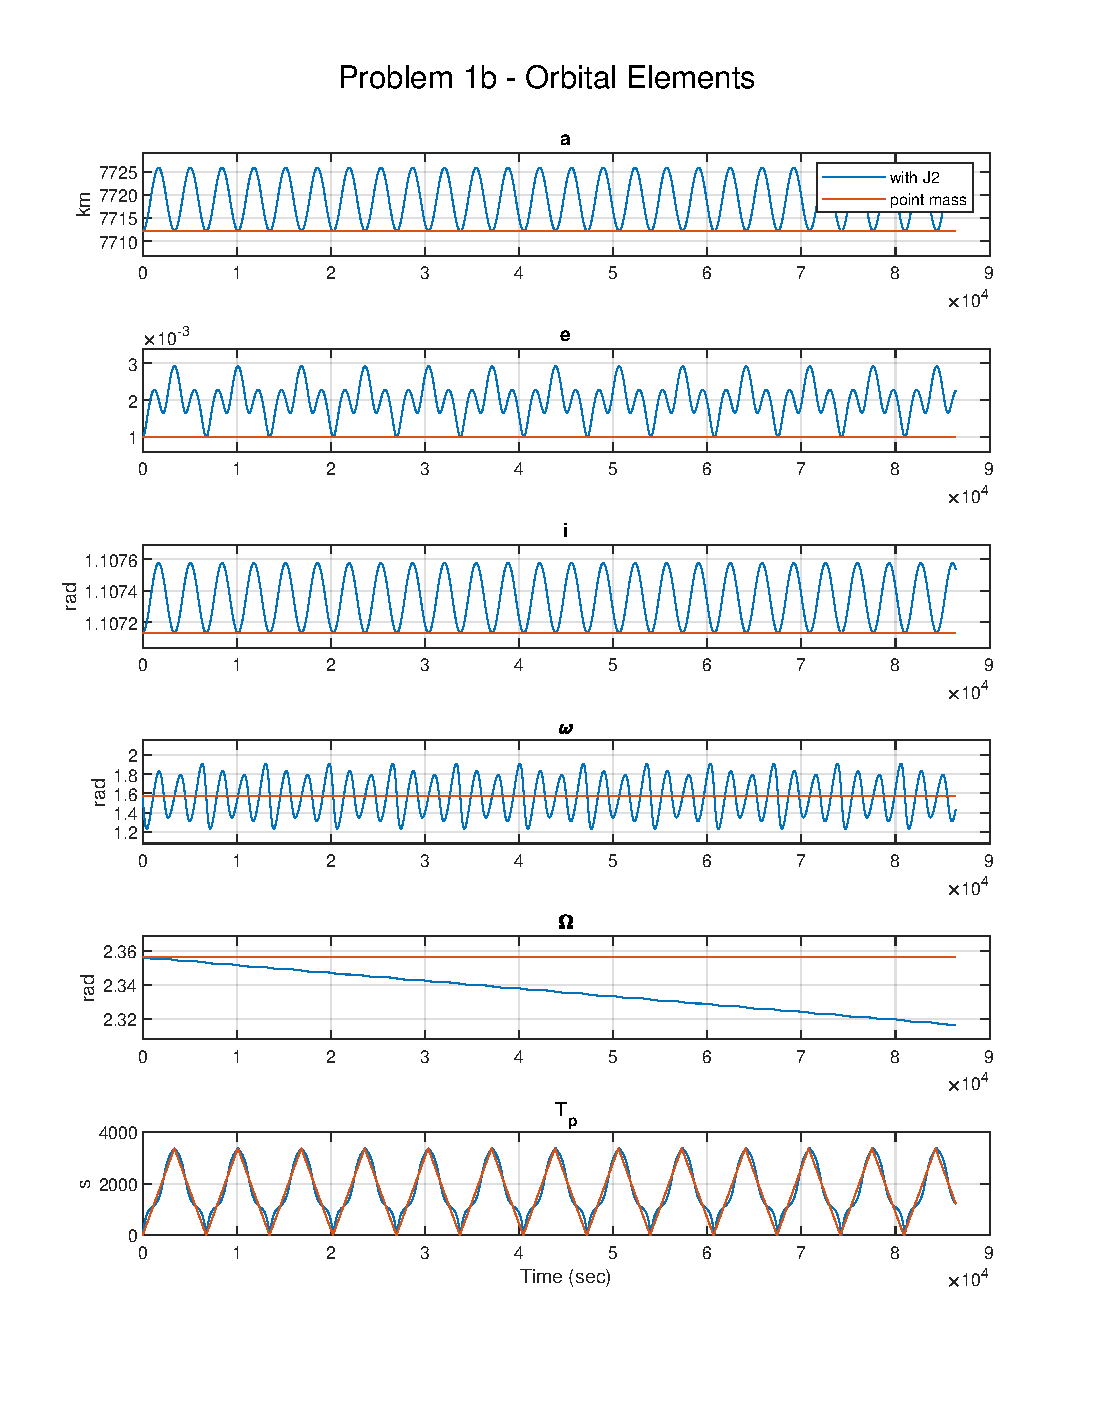
\includegraphics[width=0.8\textwidth]{Problem 1b - Orbital Elements.pdf}
	\caption{Orbital elements of point mass and point mass with J2 zonal elements} 
	\label{fig:prob_1b}	
\end{figure}

Figure \ref{fig:prob_1b} shows that the Keplerian orbital elements are remarkably stable over time. Once J2 terms were introduced, the orbit elements exhibited periodic oscillating behavior for most of the orbital elements with the exception of right ascension of the ascending node. The motion of the orbiting body in the orbital plane is planar, therefore the body will move through lines of nodes at the ascending node, where it moves from -Z to +Z in the orbit frame (in other words, the body enters the northern hemisphere from the southern hemisphere at the crossing of the ascending node) \cite{born_statorbitdet}. The linearly decreasing ramp indicates that the J2 terms perturb a constant rate effect on the node. 

The time of perigee passing has a period of approximately 6.74e3 seconds, which matches the calculation of the orbit period. The other orbit elements contain higher frequency content; perhaps these elements are likely sensitive to the J2 terms in geometric ways. In Figure \ref{fig:prob_1b_2bod}, the orbits of the point mass and point mass with modeled J2 terms is shown. The point mass orbit is very stable while the J2 orbit perturbed more and more as the day went by. 

\begin{figure}
	\centering 
	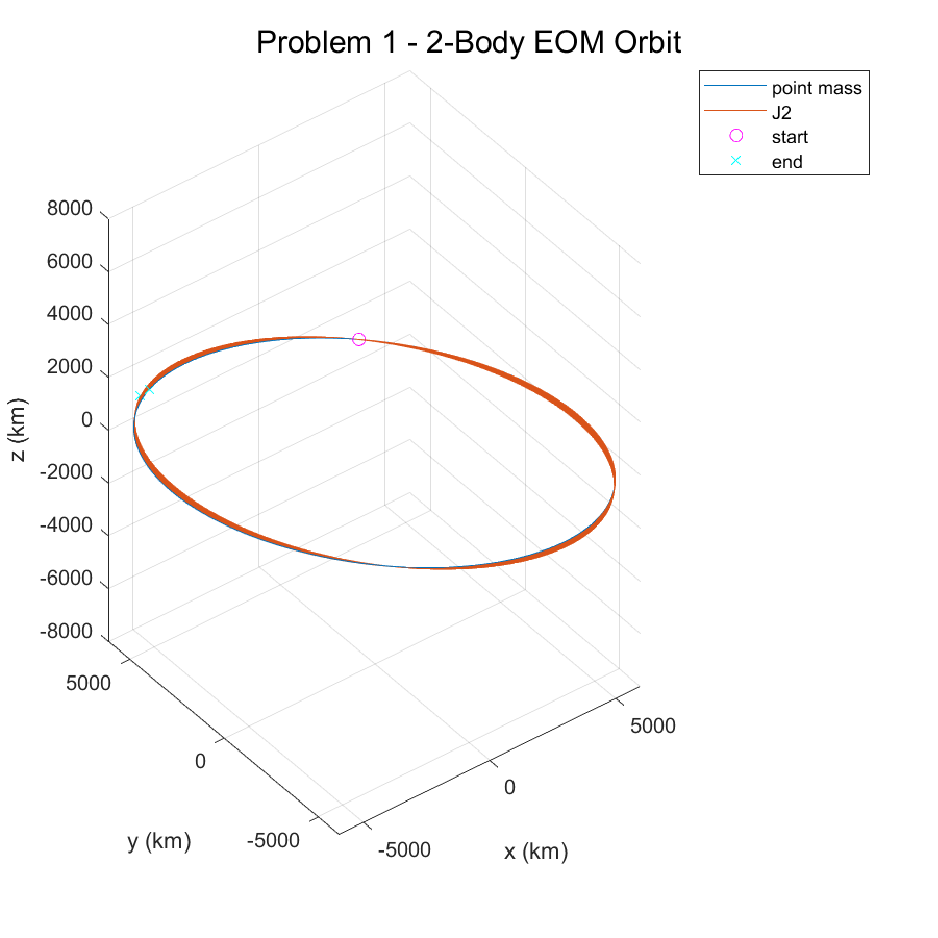
\includegraphics[width=0.8\textwidth]{Problem 1 - 2-Body EOM Orbit.pdf}
	\caption{2-body EOM Orbit of Point Mass with J2 term}
	\label{fig:prob_1b_2bod}
\end{figure}

\newpage
% ================================================================ % 

\subsection*{Problem 1c} 

 % \subsubsection*{Statement} 
\begin{center}
	\fbox{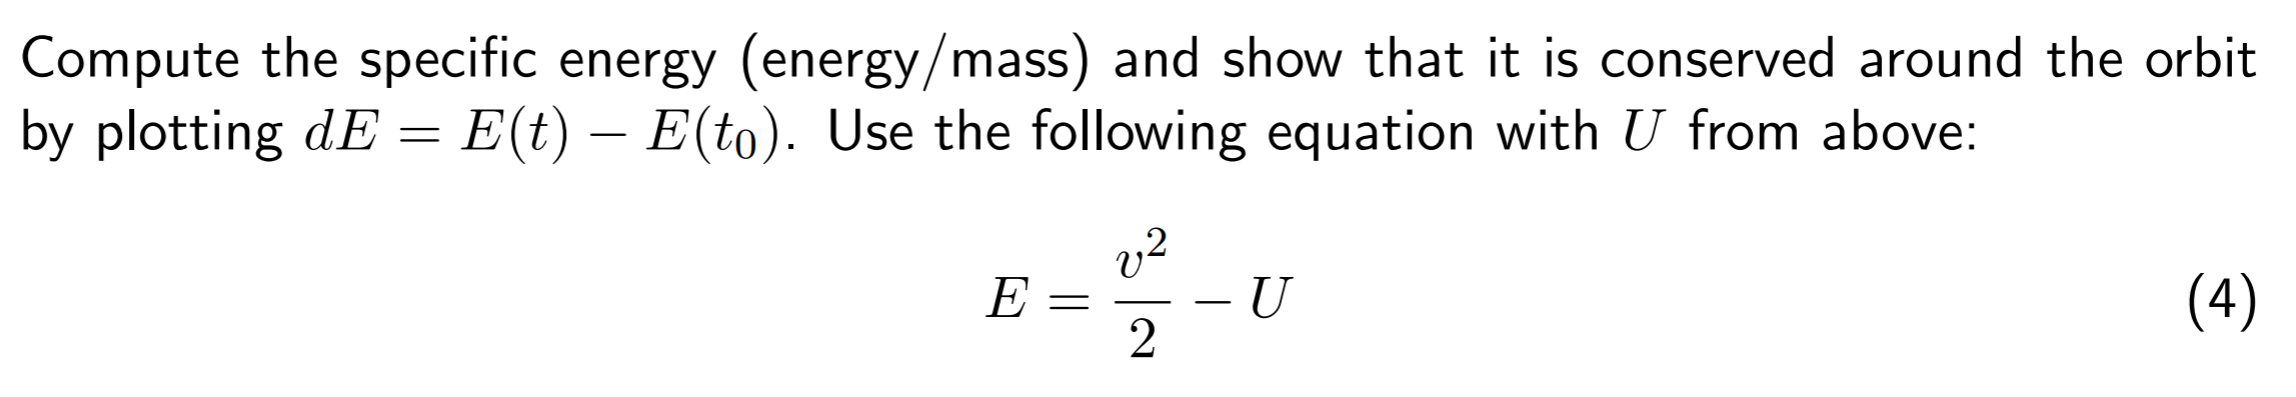
\includegraphics[width=0.9\textwidth]{prob_1c.png}} \\
\end{center}

% ---------------------------------------------------------------- % 

\subsubsection*{Solution} 

The gravitational potential function (below) was added to the magnitude of the velocity squared over 2 for each timestep of the simulation, which was specified at 20 seconds, to compute the specific energy. 

\begin{equation}
	U = U_{point mass} + U_{J_2} = \dfrac{\mu}{r} \Bigg[ 1 - J_2 \Bigg( \dfrac{R_{Earth} }{ r }^2 \Bigg) 
	\Bigg( \dfrac{3}{2} sin^2 ( \phi ) - \dfrac{1}{2} \Bigg) \Bigg]
\end{equation}

Then, to show that the specific energy is conserved, the specific energy at each timestep was subtracted with its initial value. The order of the magnitude on the plot is -12, which is a tiny change. The specific energy was around 25.815 km$^2$/s$^2$ for the duration of the simulation. 


\begin{figure}[H]
	\centering 
	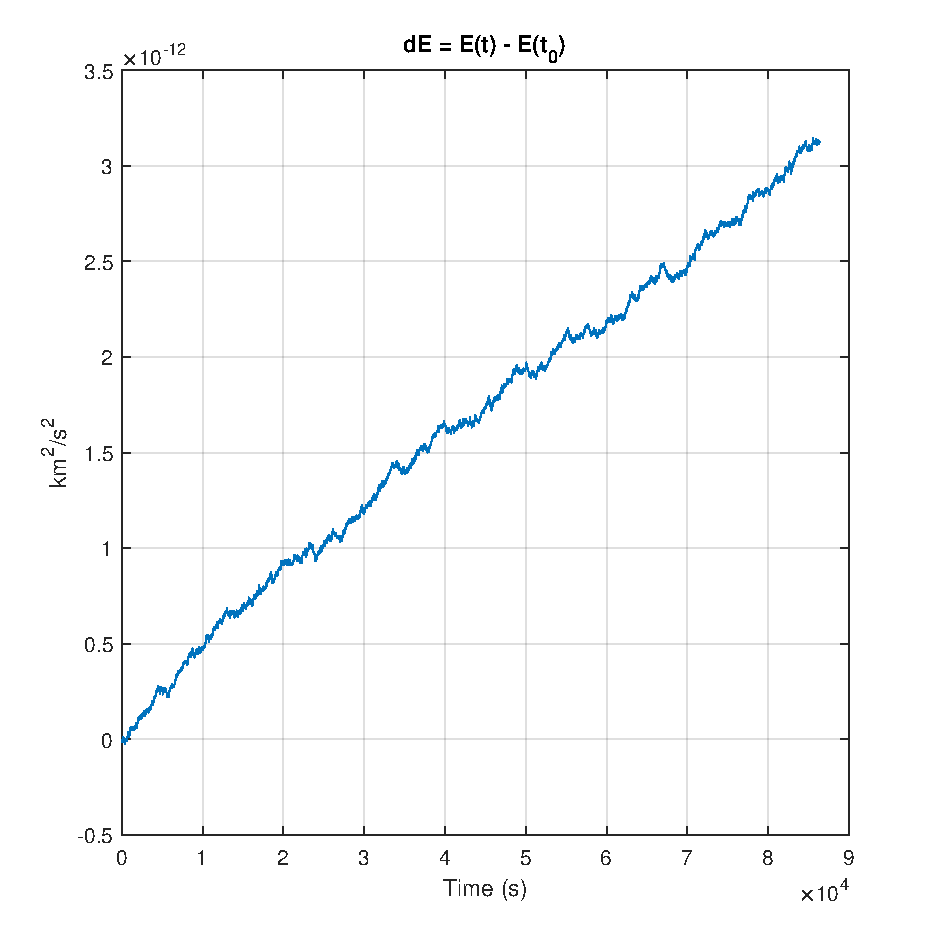
\includegraphics[width=0.8\textwidth]{Problem 1c - Delta Specific Energy.pdf}	
	\caption{Delta Specific Energy} 
	\label{fig:prob_1c}
\end{figure}


\newpage
% ================================================================ % 

\subsection*{Problem 1d} 

 % \subsubsection*{Statement} 
\begin{center}
	\fbox{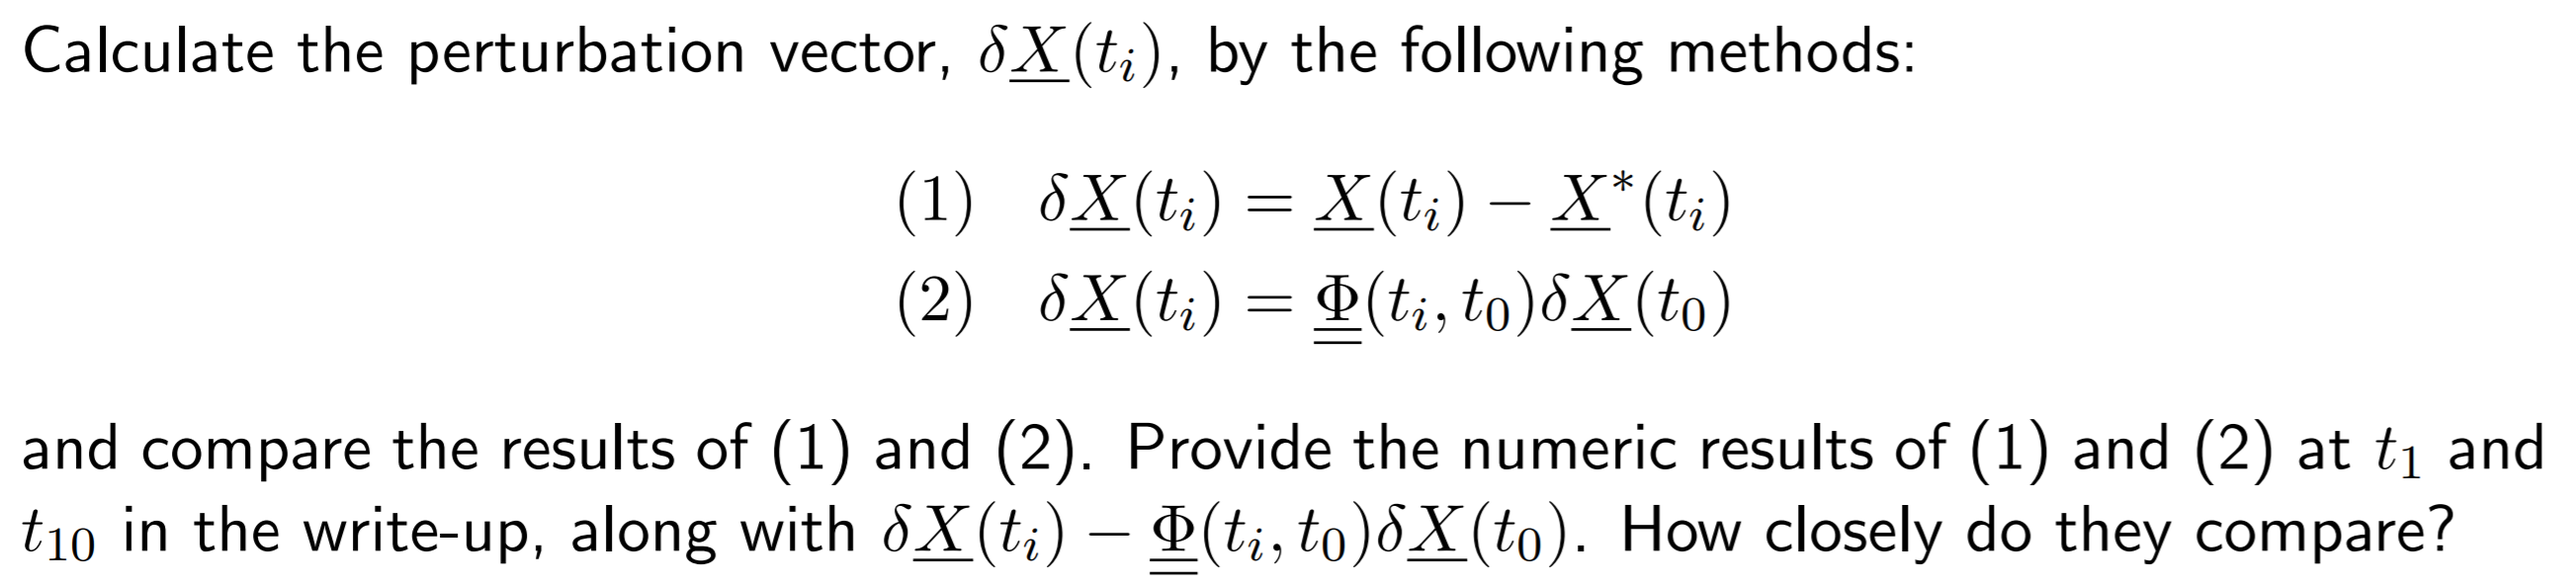
\includegraphics[width=0.9\textwidth]{prob_1d.png}} \\
\end{center}

% ---------------------------------------------------------------- % 

\subsubsection*{Solution} 

The kth-component of the (specific) angular momentum vector was also incredibly stable for the duration of the simulation. The angular momentum vector is normal to the orbit plane and is a fundamental property of the orbit frame and the conservation of orbital energy. Changing orbital energy would lead to a changing specific angular momentum vector. Although the other components of the angular momentum vector experienced periodic behavior, the kth component remained within an order of magnitude of -10 to its initial value. 

\begin{figure}[H]
	\centering 
	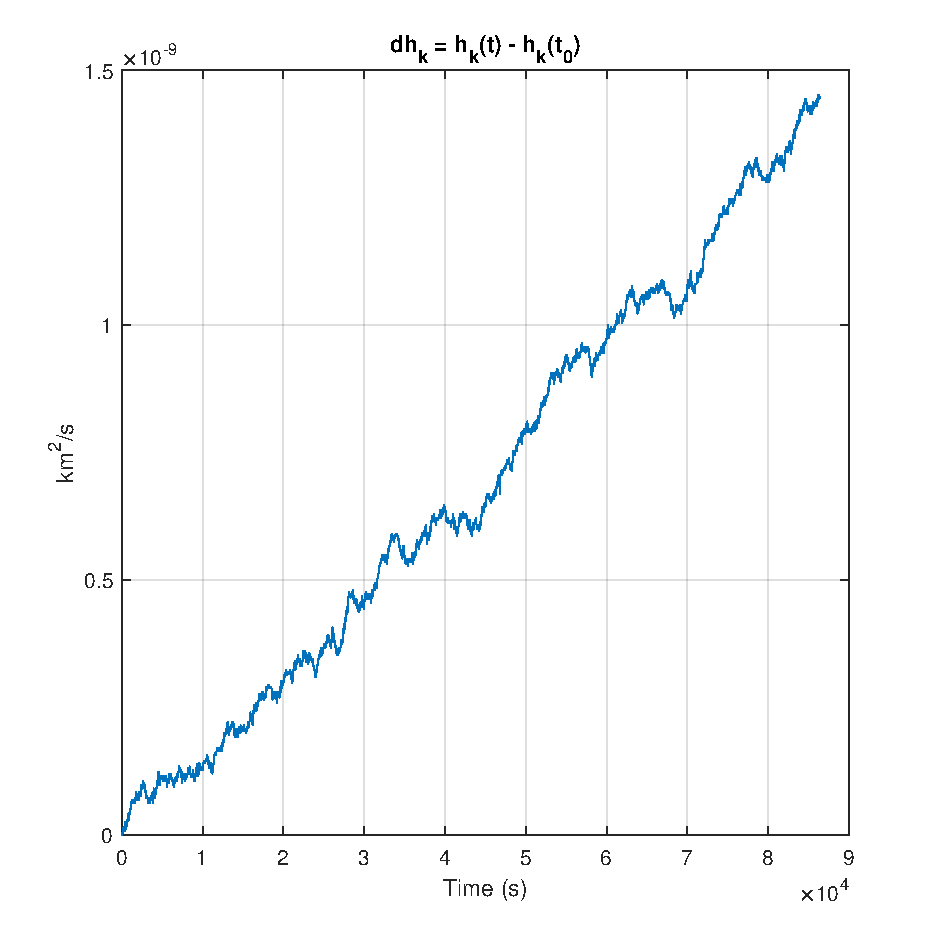
\includegraphics[width=0.8\textwidth]{Problem 1d - Delta Angular Momentum.pdf}
	\caption{Delta Angular Momentum} 
	\label{fig:prob_1d}
\end{figure}

The plot for the k component of the angular momentum vector was computed and then differenced. 



\newpage
% ================================================================ % 

\section*{Problem 2} 

 % \subsubsection*{Statement} 
\begin{center}
	\fbox{
\includegraphics[width=0.9\textwidth]{prob_2.png}} \\
\end{center}

% ---------------------------------------------------------------- % 

\subsubsection*{Solution} 




\newpage
% ================================================================ % 

\subsection*{Problem 2a} 

 % \subsubsection*{Statement} 
\begin{center}
	\fbox{
\includegraphics[width=0.9\textwidth]{prob_2a.png}} \\
\end{center}

% ---------------------------------------------------------------- % 

\subsubsection*{Solution} 

From the plot shown below, the inference that total energy is conserved can confidently be made. Specific energy is related to the angular momentum of the system, which is conserved even with the presence of drag \cite{jah_mod3}. Drag is not a conservative force, and thus does not have a significant impact on the system energy. 

\begin{figure}[H]
	\centering
	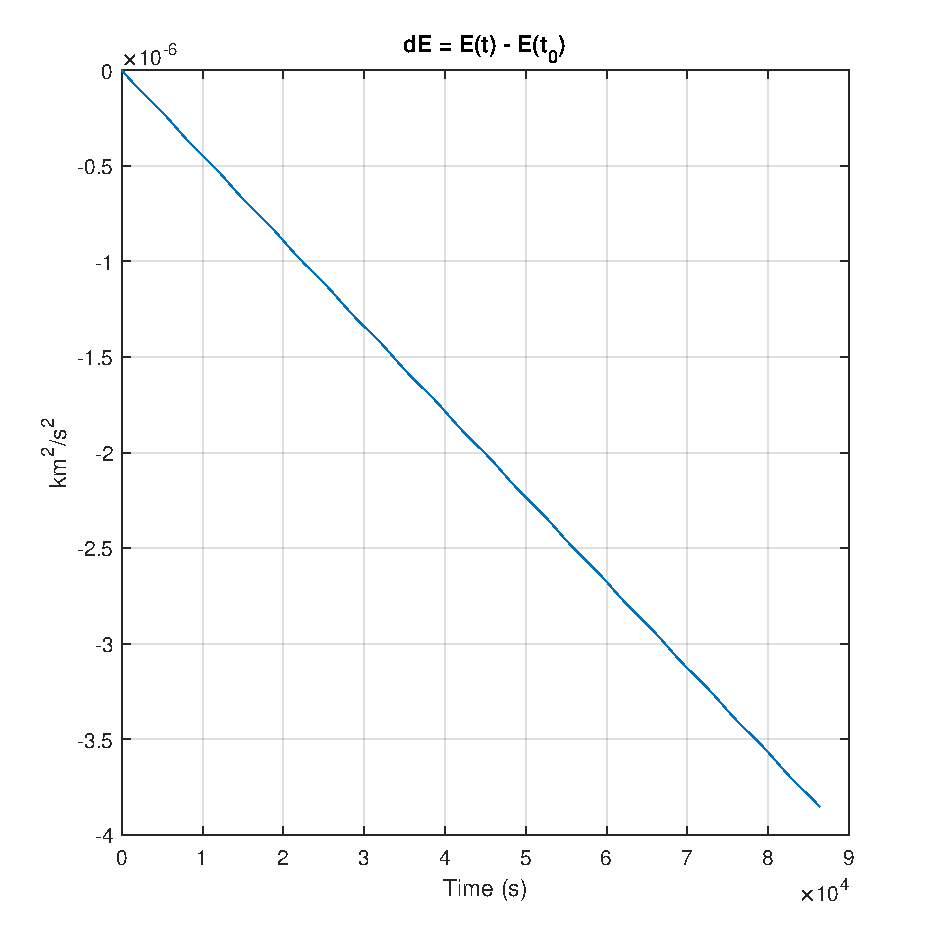
\includegraphics[width=0.8\textwidth]{Problem 2a - Delta Specific Energy.pdf}
	\caption{Delta Specific Energy for Point Mass with J2 Terms and Drag}
\end{figure}



\newpage
% ================================================================ % 

\subsection*{Problem 2b} 

 % \subsubsection*{Statement} 
\begin{center}
	\fbox{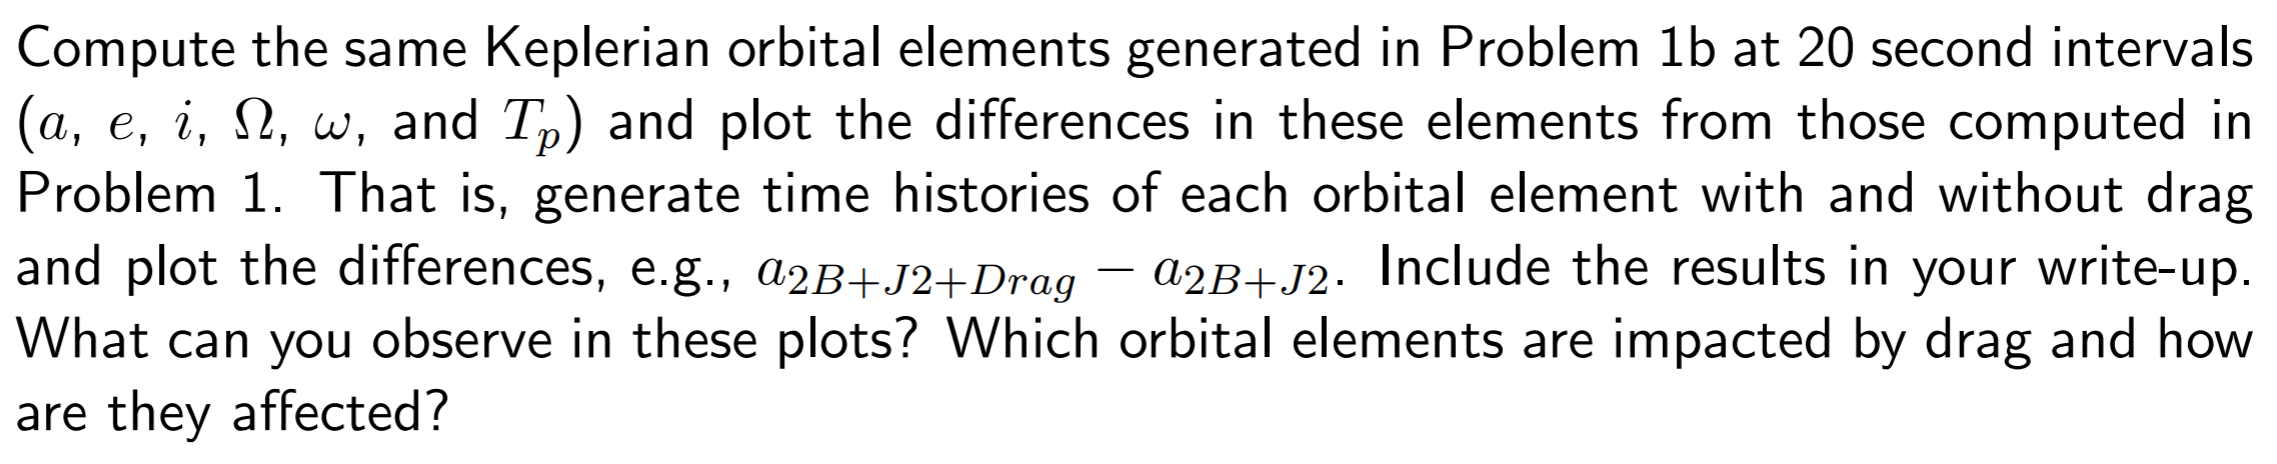
\includegraphics[width=0.9\textwidth]{prob_2b.png}} \\
\end{center}

% ---------------------------------------------------------------- % 

Results for the four cases (point mass, J2, drag, and J2 + drag) and their differences are shown below. To compare differences, there ended up being 6 delta cases analyzed: 

\begin{enumerate}
	\item point mass - J2 
	\item point mass - drag 
	\item point mass - (J2 + drag) 
	\item J2 - drag 
	\item J2 - (J2 + drag) 
	\item drag - (J2 + drag) 
\end{enumerate}

The J2 terms are extremely dominant and make it hard to discern the error between J2 and J2 + drag. The perturbation that drag ended up having on the final state of point mass is shown below (p-drag): 

\begin{table}[H]	
\begin{tabular}{|l|l|l|l|}
	\hline 
	position & -0.009913492249325 $\hat{i}$   & 0.547834133612923$\hat{j}$  & -0.776935848989524 $\hat{k}$ \\
	\hline 
	velocity & -0.000683365863896 $\hat{i}$  & 0.000451816362101$\hat{j}$   & 0.000329869465077 $\hat{k}$ \\ 
	\hline 
\end{tabular}
\end{table}
* 10$^{-8}$ 

Drag seems to have a near-negligible effect on the motion of the body. The plot of the difference between the point mass and drag is almost zero for the duration of the simulation. Drag does seem to have a slightly larger influence on right ascension of the ascending node than the other elements for this batch of runs, but the effects become far more interesting in the orbit elements plot between J2 and drag.  The time of perigee passing appears to be the most sensitive to drag; slight perturbations can be observed in the plots below. Overall, the J2 effects are clearly dominant in Figure \ref{fig:orb_j2_drag}. 

\subsubsection*{Solution} 

\begin{figure}[H]
	\centering
	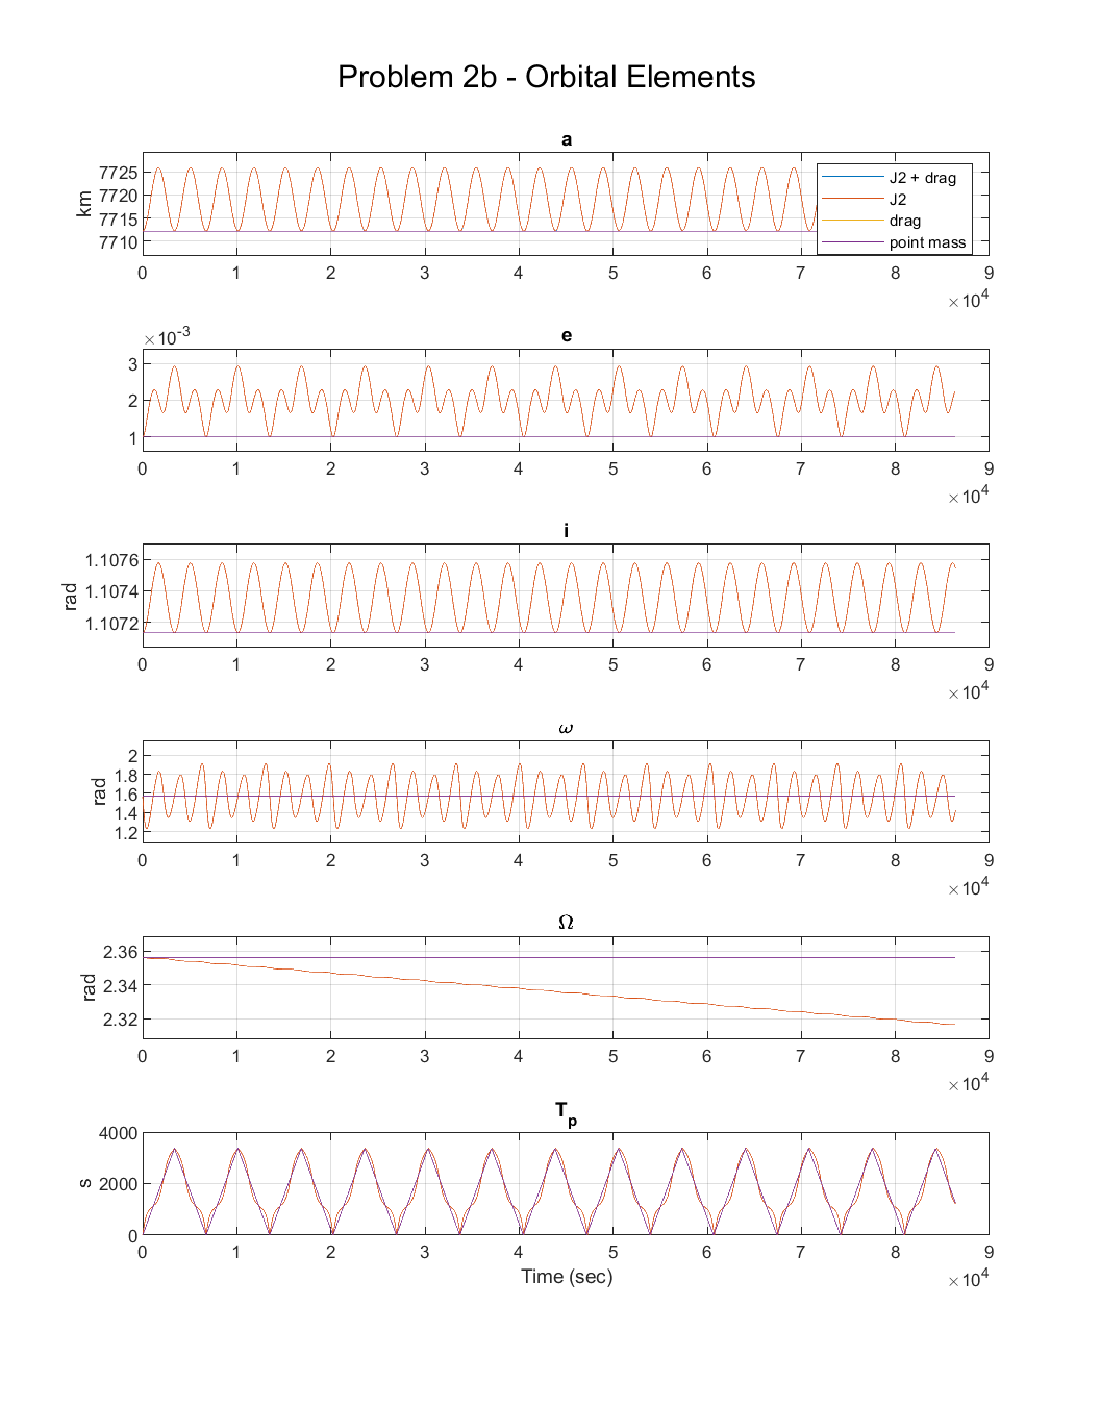
\includegraphics[width=0.8\textwidth]{Problem 2b - Orbital Elements.pdf}
	\caption{Orbital Elements for Point Mass with J2 Terms and Drag} 
\end{figure}

\begin{figure}[H]
	\centering 
	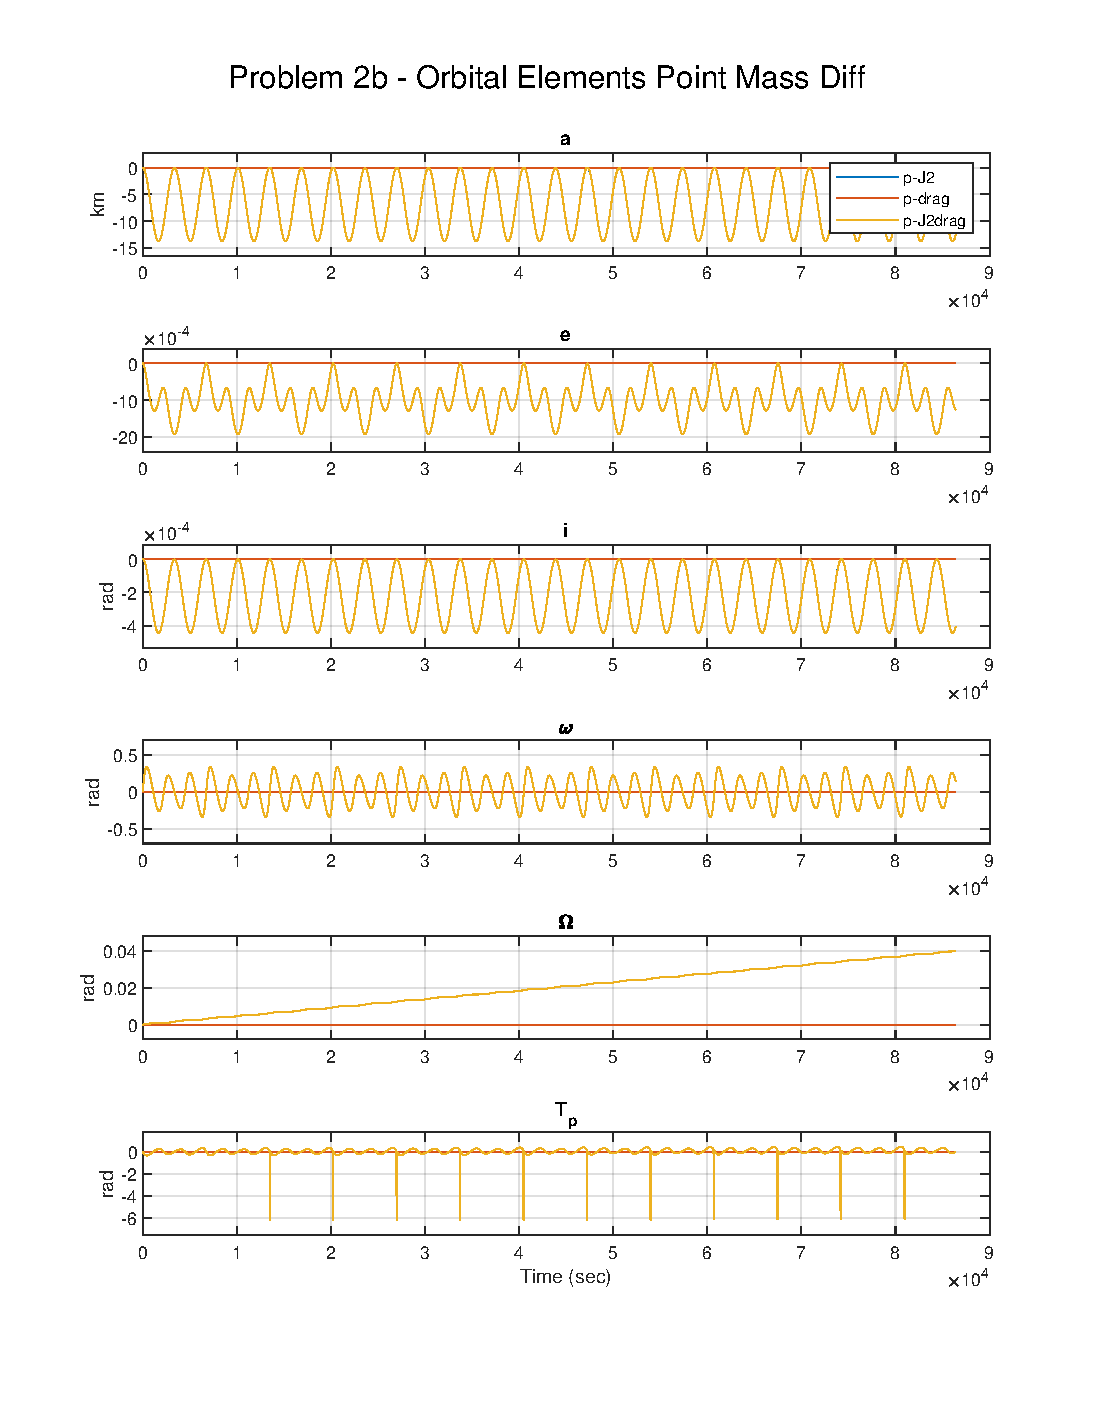
\includegraphics[width=0.8\textwidth]{Problem 2b - Orbital Elements Point Mass Diff.pdf}
	\caption{Orbital Elements Point Mass Difference} 
\end{figure}

\begin{figure}[H]
	\centering 
	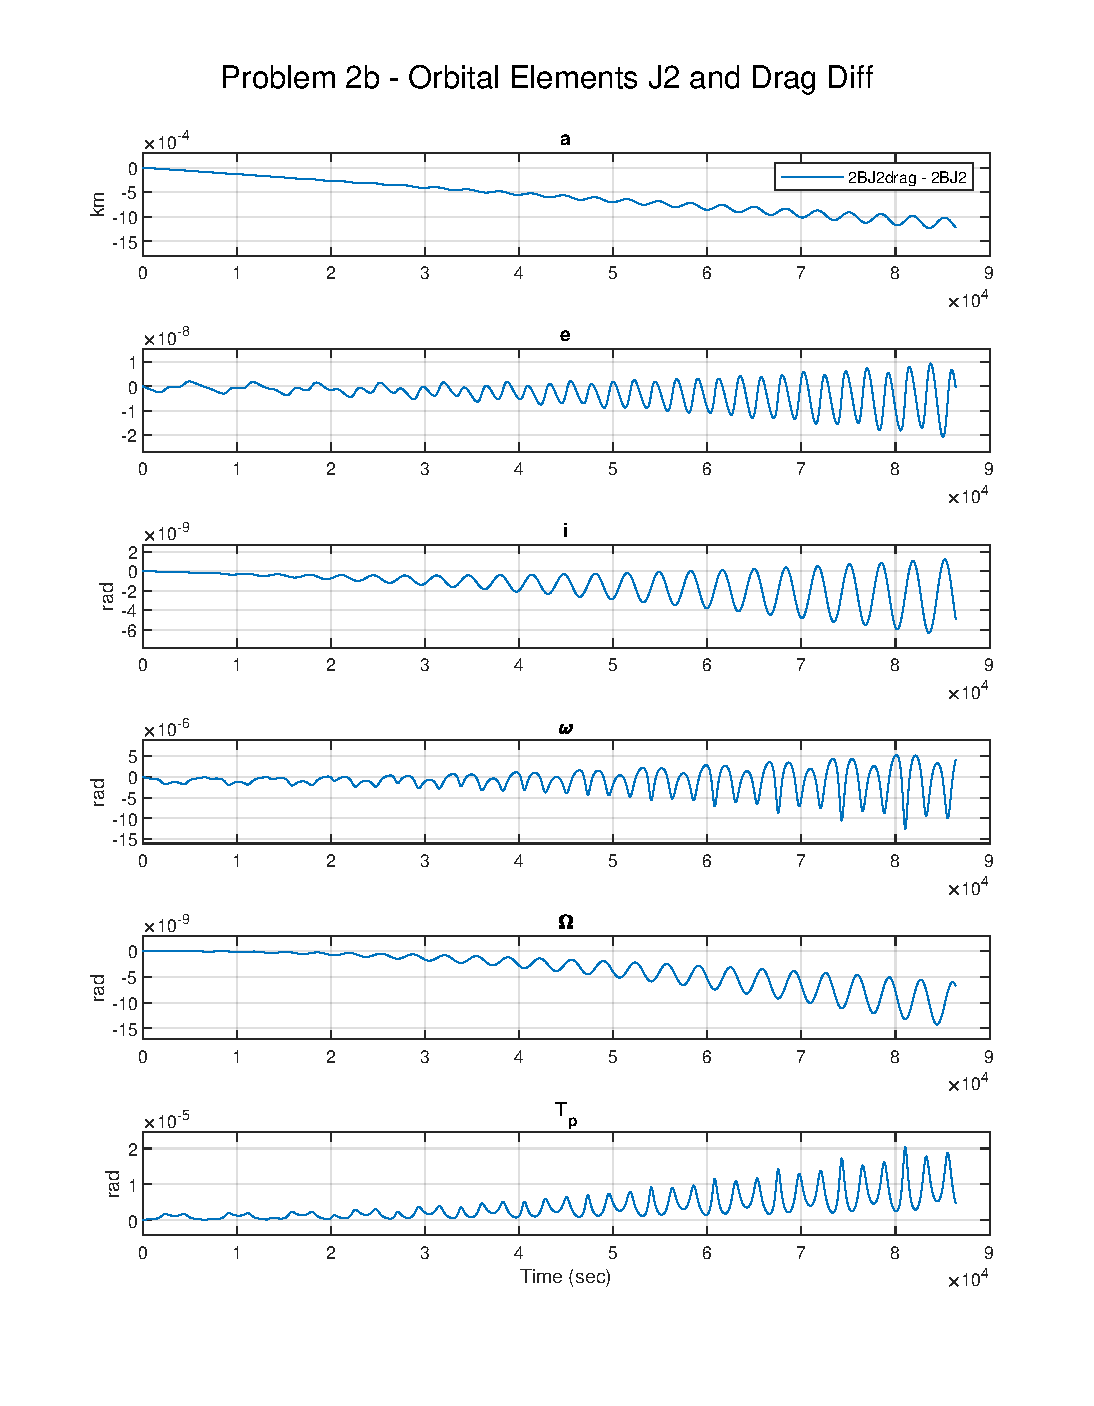
\includegraphics[width=0.8\textwidth]{Problem 2b - Orbital Elements J2 and Drag Diff.pdf}
	\caption{Orbital Elements J2 and Drag Difference} 
	\label{fig:orb_j2_drag}
\end{figure}


% ================================================================ % 

\newpage
\section*{Appendix} 

\subsection*{ $\partial U / \partial x$ derivation}

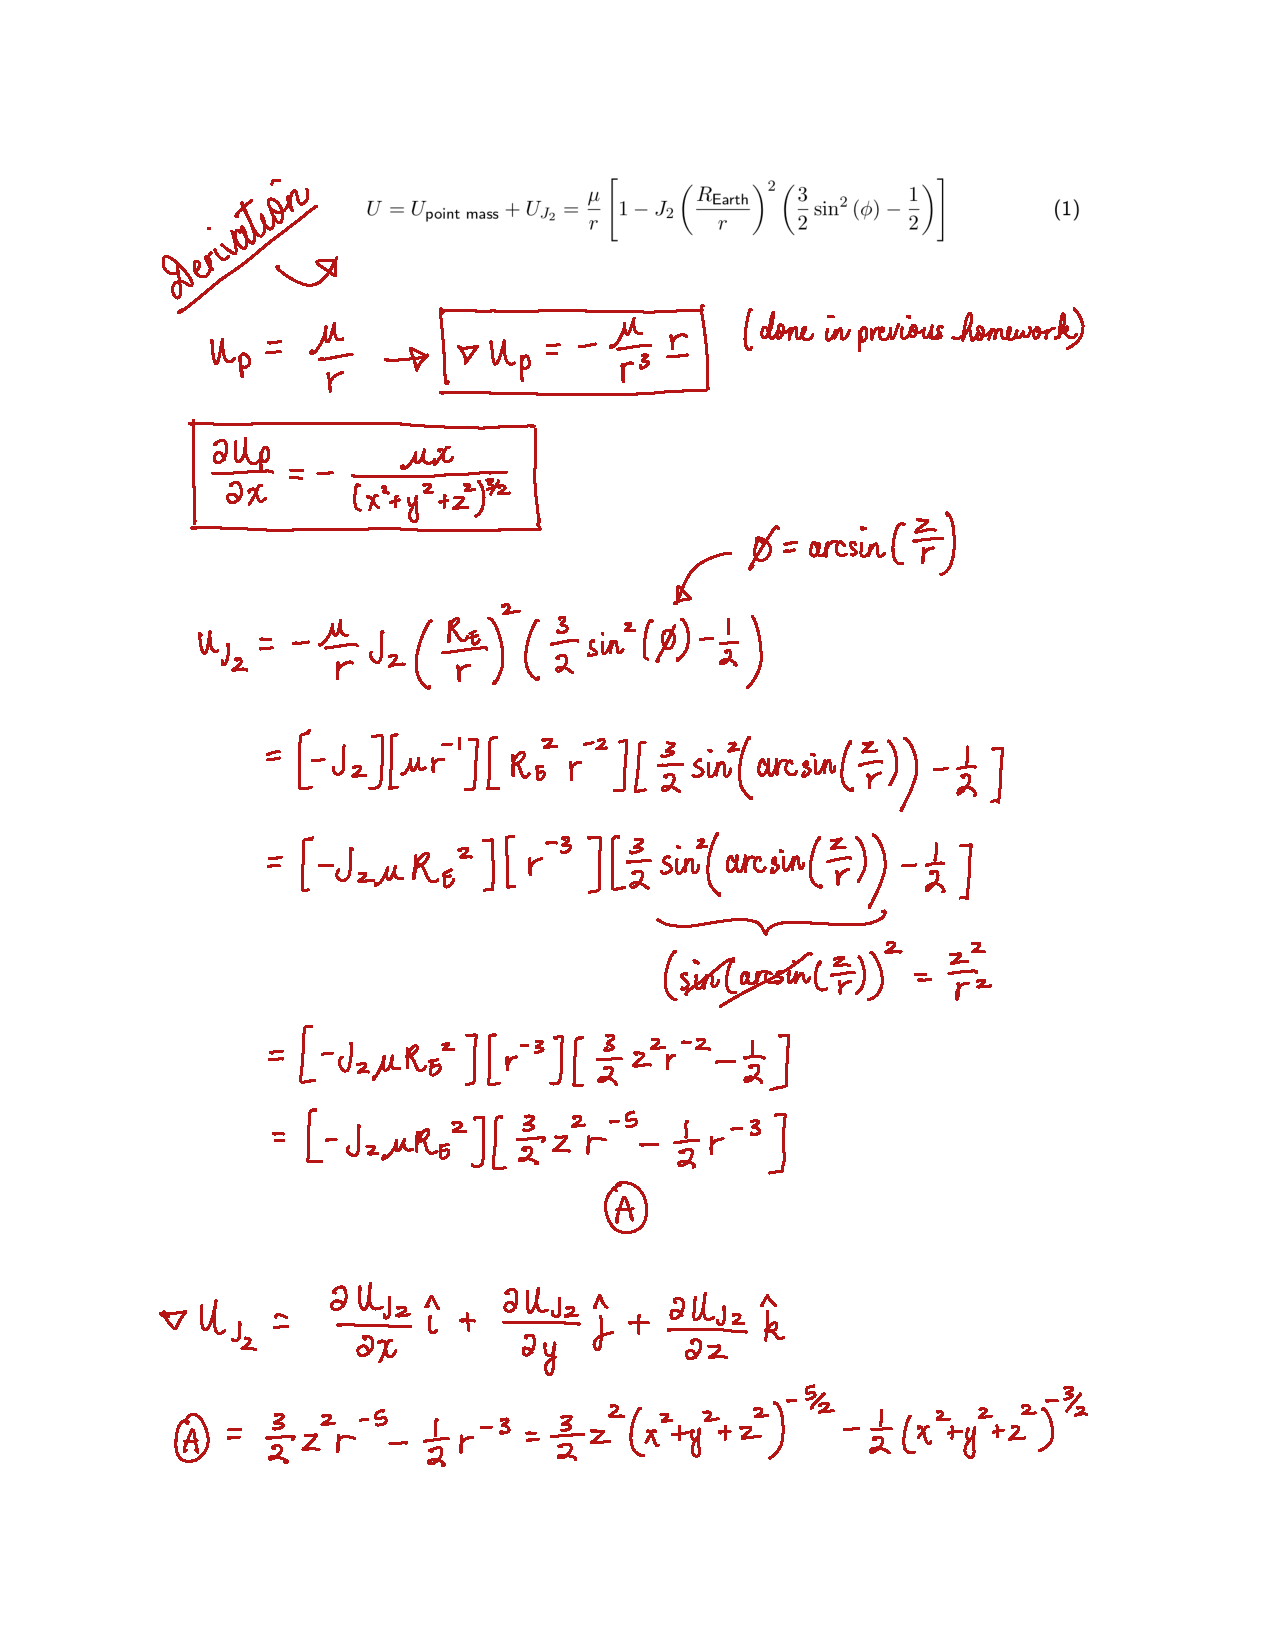
\includegraphics[page=1, width=\textwidth]{dUdx_derivation.pdf} \newpage
\includegraphics[page=2, width=\textwidth]{dUdx_derivation.pdf} \newpage
\includegraphics[page=3, width=\textwidth]{dUdx_derivation.pdf}

\newpage
\subsection*{HW2 MATLAB code} 

\begin{lstlisting}[basicstyle=\footnotesize]
% ASE 389 Orbit Determination
% HW 2
% Junette Hsin 

clear; 

positionA = [100 100 600 600]; 
positionB = [100 100 700 900]; 

%% Problem 1 

syms x y z 
global mu RE J2 

% constants 
mu = 398600.4;      % G * M1 * M2 
RE = 6378.145;      % Earth radius 
J2 = 0.00108248;    % J2 

% testing 
% syms mu RE J2 

% radius 
r = sqrt(x^2 + y^2 + z^2); 

% U point mass 
Up = mu/r; 

% latitude 
phi = asin(z/r); 

% U J2 
UJ2 = -mu/r * J2 * (RE/r)^2 * ( 3/2 * ( sin(phi) )^2 - 1/2 ); 

% gradient 
d_UJ2 = gradient(UJ2, [x y z]); 
d_UJ2 = simplify(d_UJ2); 

% Initial conditions (km)
r0  = [ -2436.45; -2436.45; 6891.037 ]; 
v0  = [ 5.088611; -5.088611; 0 ]; 
rv0 = [r0; v0]; 

% orbital elements (and sanity check) 
oe0 = rv2oe(rv0);
rv_check2 = oe2rv(oe0); 
[oe_check, oe_extra] = rv2orb_OG(rv0);  
[rv_check] = orb2rv_OG(oe_check, oe_extra); 

% 1 day period 
% a = oe(1); 
% T = abs(2 * pi * sqrt(a^3 / mu));        % period 
T = 60 * 60 * 24; 
dt = 20; 

% set ode45 params 
rel_tol = 1e-14;         % 1e-14 accurate; 1e-6 coarse 
abs_tol = 1e-16; 
options = odeset('reltol', rel_tol, 'abstol', abs_tol ); 

% INTEGRATE! Point mass and J2 
[t_p, x_p] = ode45(@TwoBod_6states, [0:dt:T], [r0; v0], options); 
[t_J2, x_J2] = ode45(@TwoBod_UJ2, [0:dt:T], [r0; v0], options); 

% ------------------------------------------------------------------------

name = 'Problem 1 - 2-Body EOM Orbit'; 
h = figure('name', name, 'position', positionA + [50 0 0 0]); 

x = x_p; 
plot3(x(:,1), x(:,2), x(:,3)); hold on; grid on; 
x = x_J2; 
plot3(x(:,1), x(:,2), x(:,3)); hold on; grid on; 

x = x_p; 
plot3(x(1,1), x(1,2), x(1,3), 'mo')
plot3(x(end,1), x(end,2), x(end,3), 'cx') 

x = x_J2; 
plot3(x(1,1), x(1,2), x(1,3), 'mo')
plot3(x(end,1), x(end,2), x(end,3), 'cx') 

legend('point mass', 'J2', 'start', 'end')

xlabel('x (km)')
ylabel('y (km)') 
zlabel('z (km)') 
%     legend('orbit', 'start', 'end')

sgtitle(name) 
save_pdf(h, name); 

%% problem 1b 

clear oe oe_check oe_p Tp_p Tp_pJ2 oe_pJ2 

for i = 1:length(x_p) 
[oe_p(i, :), Tp_p(i,:)] = rv2oe( x_p(i, :) ); 
oe_check(i, :) = rv2orb_OG( x_p(i, :) ); 
%     Tp_p(i,:) = perigee_pass(oe_p(i,:), x_p(i,:)); 
end 


for i = 1:length(x_J2)
oe_J2(i,:) = rv2oe( x_J2(i, :) ); 
oe_check(i,:) = rv2orb_OG( x_J2(i, :) ); 

Tp_J2(i,:) = perigee_pass(oe_J2(i,:), x_J2(i,:)); 
end 

% Time of perigee passage 
% n = mean motion = sqrt(mu/a^3)
% E = acos( r/a * cos(nu) + e )
% M = mean anomaly = E - e*sin(E)
% Tp = t0 - M/n 

% ------------------------------------------------------------------------

labels = {'a', 'e', 'i', '\omega', '\Omega', 'T_p'}; 
units = {'km', '', 'rad', 'rad', 'rad', 'rad'}; 
name = 'Problem 1b - Orbital Elements'; 
h = figure('name', name, 'position', positionB + [50 0 0 0]); 
for i = 1:5
subplot(6,1,i) 
plot(t_J2, oe_J2(:, i)); hold on; grid on; 
plot(t_p, oe_p(:, i)); 
title(labels{i}); 
ylabel(units{i}); 
increase_ylim; 
if i == 1
legend('with J2', 'point mass'); 
end 
end 
subplot(6,1,6) 
plot(t_J2, Tp_J2); hold on; grid on; 
plot(t_p, Tp_p); 
title('T_p') 
ylabel('s') 
sgtitle(name) 
xlabel('Time (sec)') 
save_pdf(h, name); 

%% Problem 1c: energy 

clear vnorm 
clear h 
clear h_mom 
clear dE 
clear dh 
clear dhnorm 

for i = 1:length(x_J2)

U(:,i) = comp_U(x_J2(i, 1:3)); 
vnorm(:,i) = sqrt( x_J2(i,4)^2 + x_J2(i,5)^2 + x_J2(i,6)^2 ); 
E(:,i) = vnorm(:,i)^2 / 2 - U(:,i); 
a = [ x_J2(i,1), x_J2(i,2), x_J2(i,3) ]; 
b = [ x_J2(i,4), x_J2(i,5), x_J2(i,6) ]; 
h_mom(:,i) = cross( a , b ); 

dE(:,i) = E(i) - E(1); 
dh(:,i) = h_mom(:,i) - h_mom(:,1); 
dhnorm(:,i) = norm( dh(:,i) ); 

end 

% ------------------------------------------------------------------------

name = 'Problem 1c - Delta Specific Energy'; 
h = figure('name', name, 'position', positionA + [50 0 0 0]); 
plot(t_J2, dE); 
title( 'dE = E(t) - E(t_0)' ) 
xlabel('Time (s)') 
ylabel('km^2/s^2') 
save_pdf(h, name); 


%% Problem 1d: angular momentum 


name = 'Problem 1d - Delta Angular Momentum'; 
h = figure('name', name, 'position', positionA + [50 0 0 0]); 
plot(t_J2, dh(3, :)); 
title( 'dh_k = h_k(t) - h_k(t_0)' ) 
xlabel('Time (s)') 
ylabel('km^2/s') 
save_pdf(h, name); 


%% Problem 2: DRAG 

global CD A m p0 r0_drag H dtheta 

CD = 2; 
A = 3.6e-6; % --> km^2 
m = 1350; 
p0 = 4e-4; % --> -13 --> -4, multiply 1e9 when going 1/m^3 to 1/km^3  
r0_drag = 7298.145; 
H = 200; 
dtheta = 7.29211585530066e-5; 

% set 1 day period (again just in case) 
T = 60 * 60 * 24; 

% set ode45 params 
rel_tol = 1e-14;         % 1e-14 accurate; 1e-6 coarse 
abs_tol = 1e-16; 
options = odeset('reltol', rel_tol, 'abstol', abs_tol ); 

% INTEGRATE! Point mass and J2 and drag 
[t_J2drag, x_J2drag] = ode45(@TwoBod_UJ2_drag, [0:dt:T], [r0; v0], options); 

% INTEGRATE! Point mass and drag 
[t_drag, x_drag] = ode45(@TwoBod_drag, [0:dt:T], [r0; v0], options); 


%% Problem 2a: specific energy 


clear vnorm 
clear h 
clear h_mom 
clear dE 
clear dh 
clear dhnorm 

for i = 1:length(x_J2drag)

U(:,i) = comp_U(x_J2drag(i, 1:3)); 
vnorm(:,i) = sqrt( x_J2drag(i,4)^2 + x_J2drag(i,5)^2 + x_J2drag(i,6)^2 ); 
E(:,i) = vnorm(:,i)^2 / 2 - U(:,i); 
a = [ x_J2drag(i,1), x_J2drag(i,2), x_J2drag(i,3) ]; 
b = [ x_J2drag(i,4), x_J2drag(i,5), x_J2drag(i,6) ]; 
h_mom(:,i) = cross( a , b ); 

dE(:,i) = E(i) - E(1); 
dh(:,i) = h_mom(:,i) - h_mom(:,1); 
dhnorm(:,i) = norm( dh(:,i) ); 

end 

% ------------------------------------------------------------------------

name = 'Problem 2a - Delta Specific Energy'; 
h = figure('name', name, 'position', positionA + [50 0 0 0]); 
plot(t_J2drag, dE); 
title( 'dE = E(t) - E(t_0)' ) 
xlabel('Time (s)') 
ylabel('km^2/s^2') 
save_pdf(h, name); 

%% Problem 2b: orbital elements 


clear oe_drag Tp_drag 

for i = 1:length(x_drag) 
[oe_drag(i, :), Tp_drag(i,:)] = rv2oe( x_drag(i, :) ); 
oe_check(i, :) = rv2orb_OG( x_p(i, :) ); 
%     Tp_p(i,:) = perigee_pass(oe_p(i,:), x_p(i,:)); 
end 

for i = 1:length(x_J2drag) 
[oe_J2drag(i, :), Tp_J2drag(i,:)] = rv2oe( x_J2drag(i, :) ); 
oe_check(i, :) = rv2orb_OG( x_p(i, :) ); 
end 

% ------------------------------------------------------------------------

labels = {'a', 'e', 'i', '\omega', '\Omega', 'T_p'}; 
units = {'km', '', 'rad', 'rad', 'rad', 'rad'}; 
name = 'Problem 2b - Orbital Elements'; 
h = figure('name', name, 'position', positionB + [50 0 0 0]); 
for i = 1:5
subplot(6,1,i) 
plot(t_J2drag, oe_J2drag(:,i)); hold on; grid on;
plot(t_J2, oe_J2(:, i));  
plot(t_drag, oe_drag(:, i)); 
plot(t_p, oe_p(:, i)); 
title(labels{i}); 
ylabel(units{i}); 
increase_ylim; 
if i == 1
legend('J2 + drag', 'J2', 'drag', 'point mass'); 
end 
end 
subplot(6,1,6) 
plot(t_J2drag, Tp_J2drag); hold on; grid on; 
plot(t_J2, Tp_J2); 
plot(t_drag, Tp_drag); 
plot(t_p, Tp_p); 
title('T_p') 
ylabel('s') 
sgtitle(name) 
xlabel('Time (sec)') 
save_pdf(h, name); 



% ------------------------------------------------------------------------
% differences in orbital elements 

% 6 combinations: 
% (1) p - J2 
% (2) p - drag 
% (3) p - J2drag 
% (4) J2 - drag 
% (5) J2 - J2drag 
% (6) drag - J2drag 

% add Tp, make your life easier 

oe_p = [oe_p, Tp_p]; 
oe_J2 = [oe_J2, Tp_J2]; 
oe_J2drag = [oe_J2drag, Tp_J2drag]; 
oe_drag = [oe_drag, Tp_drag]; 

p_J2 = oe_p - oe_J2; 
p_drag = oe_p - oe_drag; 
p_J2drag = oe_p - oe_J2drag; 
J2_drag = oe_J2 - oe_drag; 
J2_J2drag = oe_J2 - oe_J2drag; 
drag_J2drag = oe_drag - oe_J2drag; 

labels = {'a', 'e', 'i', '\omega', '\Omega', 'T_p', 'T_p'}; 
units = {'km', '', 'rad', 'rad', 'rad', 'rad', 's'}; 
name = 'Problem 2b - Orbital Elements Point Mass Diff'; 
h = figure('name', name, 'position', positionB + [50 0 0 0]); 
for i = 1:6
subplot(6,1,i) 
plot(t_J2, p_J2(:,i)); hold on; grid on; 
plot(t_J2, p_drag(:,i));
plot(t_J2, p_J2drag(:,i)); 

title(labels{i}); 
ylabel(units{i}); 
increase_ylim; 
if i == 1
legend('p-J2', 'p-drag', 'p-J2drag'); 
end 
end 
sgtitle(name) 
xlabel('Time (sec)') 
save_pdf(h, name); 

labels = {'a', 'e', 'i', '\omega', '\Omega', 'T_p', 'T_p'}; 
units = {'km', '', 'rad', 'rad', 'rad', 'rad', 's'}; 
name = 'Problem 2b - Orbital Elements J2 and Drag Diff'; 
h = figure('name', name, 'position', positionB + [50 0 0 0]); 
for i = 1:6
subplot(6,1,i) 
plot(t_J2, J2_drag(:,i)); hold on; grid on; 
plot(t_J2, J2_J2drag(:,i)); 
plot(t_J2, drag_J2drag(:,i)); 

title(labels{i}); 
ylabel(units{i}); 
increase_ylim; 
if i == 1
legend('J2-drag', 'J2-J2drag', 'drag-J2drag'); 
end 
end 
sgtitle(name) 
xlabel('Time (sec)') 
save_pdf(h, name); 



%%     
%% subfunctions 

function save_pdf(h, name) 

% save as cropped pdf 
set(h,'Units','Inches');
pos = get(h,'Position');
set(h,'PaperPositionMode','Auto','PaperUnits','Inches','PaperSize',[pos(3), pos(4)])
print(h,name,'-dpdf','-r0')

end 

function increase_ylim

ylims  = get(gca, 'ylim');
yd     = ylims(2) - ylims(1); 
set(gca, 'ylim', [ylims(1) - 0.2*yd, ylims(2) + 0.2*yd  ]); 

end 

function U = comp_U(rv) 

global mu J2 RE 

x = rv(1); 
y = rv(2); 
z = rv(3); 

% radius 
r = sqrt(x^2 + y^2 + z^2); 

% U point mass 
Up = mu/r; 

% latitude 
phi = asin(z/r); 

% U J2 
UJ2 = -mu/r * J2 * (RE/r)^2 * ( 3/2 * ( sin(phi) )^2 - 1/2 ); 

% U point mass 
U = Up + UJ2; 

end 

function Tp = perigee_pass(oe, x) 

global mu 

% perigee passing 
a = oe(1); 
e = oe(2); 
nu = oe(6); 
%     r = norm([ x_pJ2(i,1) x_pJ2(i,2) x_pJ2(i,3) ]); 
r = sqrt( x(1)^2 + x(2)^2 + x(3)^2 ); 

n = sqrt(mu/a^3); 
E = acos( r/a * cos(nu) + e );
M = E - e*sin(E); 
Tp = M/n; 

end 



\end{lstlisting}

\subsection*{rv2oe function}

\begin{lstlisting}[basicstyle=\footnotesize]
function [oe, Tp] = rv2oe(rv)
% ------------------------------------------------------------------------
% Inputs 
%   rv = [6x1] position and velocity states vector in ECI frame 
% 
% Outputs 
%   oe = [6x1] orbital elements: a, e, i, w, Omega, nu
%           a   = semimajor axis 
%           e   = eccentricity 
%           i   = inclination 
%           w   = argument of perigee 
%           O   = right ascension of ascending node 
%           M   = mean anomaly 
%           Tp  = time of perigee passing  (optional output) 
% ------------------------------------------------------------------------

global mu 

r = rv(1:3); 
v = rv(4:6); 

% angular momentum 
h       = cross(r,v); 

% node vector 
nhat    = cross( [0 0 1], h ); 

% eccentricity 
evec    = ( (norm(v)^2 - mu/norm(r))*r - dot(r,v)*v ) / mu; 
e       = norm(evec); 

% specific mechanical energy 
energy  = norm(v)^2/2 - mu/norm(r); 

% semi-major axis and p
if abs(e-1.0)>eps
a = -mu/(2*energy); 
p = a*(1-e^2); 
else
p = norm(h)^2/mu; 
a = inf; 
end

% inclination 
i = acos(h(3)/norm(h)); 

% right ascension of ascending node (check for equatorial orbit) 
if i > 0.000001
O = acos( nhat(1)/norm(nhat) ); 
else
O = 0; 
end
if isnan(O)
O = 0; 
end
if nhat(2)<0
O = 2*pi - O; 
end

% argument of perigee 
if e > 0.000001
w = acos(dot(nhat,evec)/(norm(nhat)*e)); 
else
w = 0; 
end
if isnan(w)
w = 0; 
end
% if e(3)<0
%    argp = 360-argp
% end

% true anomaly 
nu = acos( dot(evec,r) / (e*norm(r)) );  
% if dot(r,v)<0
%    nu = 360 - nu
% end

%Apply Quadrant Checks to All Determined Angles
% idx = nhat(2) < 0; if any(idx); O(idx) = 2*pi - O(idx);  end
% idx = evec(3) < 0; if any(idx); w(idx) = 2*pi - w(idx); end
idx = dot(r,v) < 0; if any(idx); nu(idx) = 2*pi - nu(idx); end

oe = [a; e; i; w; O; nu]; 

% perigee passing time 

rnorm = norm(r); 
n = sqrt(mu/a^3); 
E = acos( rnorm/a * cos(nu) + e );
M = E - e*sin(E); 
Tp = M/n; 

end
\end{lstlisting}

\subsection*{oe2rv function}

\begin{lstlisting}
function [rv] = oe2rv(oe)
% ------------------------------------------------------------------------ 
% Purpose: Convert orbital elements and time past epoch to the classic 
% Cartesian position and velocity
% 
% Inputs: 
%   oe      = [6x1] or [1x6] orbital elements 
%   delta_t = t - t0 time interval 
%   mu      = Gravity * Mass (of Earth) constant 
% 
% Outputs: 
%   rv      = position and velocity state vector 
% ------------------------------------------------------------------------ 

% global delta_t 
global mu 

a       = oe(1); 
e       = oe(2); 
i       = oe(3); 
w       = oe(4); 
LAN     = oe(5); 
% M0      = oe(6); 
nu      = oe(6); 

% nu is TRUE ANOMALY --> use Kepler's to calculate MEAN ANOMALY 
% E = 2*atan( sqrt( (1-e)/(1+e) ) * tan(nu/2) ); 
% M = M0 + sqrt( mu/a^3 ) * (delta_t); 
% E = keplerEq(M, e, eps); 
% E = kepler(M, e); 
% nu = 2*atan( sqrt( (1+e)/(1-e) ) * tan(E/2) ); 

p = a * ( 1 - e^2 );            % intermediate variable 
r = p / ( 1 + e*cos(nu) );      % r_magnitude, polar coordinates 

% Perifocal position and velocity 

r_pf = [ r * cos(nu); r * sin(nu); 0 ]; 
v_pf = [ -sqrt(mu/p) * sin(nu); sqrt(mu/p) * (e + cos(nu)); 0 ]; 

% Perifocal to ECI transformation, 3-1-3 rotation 
R11 = cos(LAN)*cos(w) - sin(LAN)*sin(w)*cos(i); 
R12 = -cos(LAN)*sin(w) - sin(LAN)*cos(w)*cos(i); 
R13 = sin(LAN)*sin(i); 

R21 = sin(LAN)*cos(w) + cos(LAN)*sin(w)*cos(i); 
R22 = -sin(LAN)*sin(w) + cos(LAN)*cos(w)*cos(i); 
R23 = -cos(LAN)*sin(i); 

R31 = sin(w)*sin(i); 
R32 = cos(w)*sin(i); 
R33 = cos(i); 

R = [R11 R12 R13; R21 R22 R23; R31 R32 R33]; 

% Transform perifocal to ECI frame 
r_vec = R * r_pf; 
v_vec = R * v_pf; 

% Position and state vector 
rv = [r_vec; v_vec]; 

end 

%% Kepler equation solvers 

function E = keplerEq(M,e,eps)
% Function solves Kepler's equation M = E-e*sin(E)
% Input - Mean anomaly M [rad] , Eccentricity e and Epsilon 
% Output  eccentric anomaly E [rad]. 
En  = M;
Ens = En - (En-e*sin(En)- M)/(1 - e*cos(En));
while ( abs(Ens-En) > eps )
En = Ens;
Ens = En - (En - e*sin(En) - M)/(1 - e*cos(En));
end
E = Ens;
end

function E = kepler(M, e)
f = @(E) E - e * sin(E) - M;
E = fzero(f, M);  % <-- I would use M as the initial guess instead of 0
end
\end{lstlisting}

\subsection*{Integrated Equations of Motion} 

\begin{lstlisting}

function dx = TwoBod_6states(t, x)
% ------------------------------------------------------------------------
% Inputs 
%   t = [Nx1] time vector (orbit is Keplerian, doesn't matter) 
%   x = [6x1] state vector 
% 
% Outputs 
%   dx = [6x1] derivative of state vector 
% ------------------------------------------------------------------------

global mu 

dx = zeros(6, 1);   % force column vector 

dx(1:3) = x(4:6); 
% r_norm  = sqrt( x(1)^2 + x(2)^2 + x(3)^2 ); 
r_norm  = norm(x(1:3)); 
dx(4:6) = ( - mu / r_norm^3 ) * x(1:3); 

end 

function dx = TwoBod_UJ2(t, x)
% ------------------------------------------------------------------------
% Inputs 
%   t = [Nx1] time vector (orbit is Keplerian, doesn't matter) 
%   x = [6x1] state vector 
% 
% Outputs 
%   dx = [6x1] derivative of state vector 
% ------------------------------------------------------------------------

global mu J2 RE 

dx = zeros(6, 1);   % force column vector 

dx(1:3) = x(4:6); 
% r_norm  = sqrt( x(1)^2 + x(2)^2 + x(3)^2 ); 
r_norm  = norm(x(1:3)); 
dx(4:6) = ( - mu / r_norm^3 ) * x(1:3); 

% J2 stuff 
dUx =      -(3*J2*RE^2*mu*x(1)*(x(1)^2 + x(2)^2 - 4*x(3)^2)) / (2*(x(1)^2 + x(2)^2 + x(3)^2)^(7/2)); 
dUy =      -(3*J2*RE^2*mu*x(2)*(x(1)^2 + x(2)^2 - 4*x(3)^2)) / (2*(x(1)^2 + x(2)^2 + x(3)^2)^(7/2)); 
dUz =  -(3*J2*RE^2*mu*x(3)*(3*x(1)^2 + 3*x(2)^2 - 2*x(3)^2)) / (2*(x(1)^2 + x(2)^2 + x(3)^2)^(7/2)); 

dx(4:6) = dx(4:6) + [dUx; dUy; dUz]; 

end 

function dx = TwoBod_UJ2(t, x)
% ------------------------------------------------------------------------
% Inputs 
%   t = [Nx1] time vector (orbit is Keplerian, doesn't matter) 
%   x = [6x1] state vector 
% 
% Outputs 
%   dx = [6x1] derivative of state vector 
% ------------------------------------------------------------------------

global mu J2 RE 
global CD A m p0 r0_drag H dtheta 

dx = zeros(6, 1);   % force column vector 

dx(1:3) = x(4:6); 
% r_norm  = sqrt( x(1)^2 + x(2)^2 + x(3)^2 ); 
rnorm  = norm(x(1:3)); 
dx(4:6) = ( - mu / rnorm^3 ) * x(1:3); 

% drag stuff 
pA = p0 * exp( -(rnorm - r0_drag)/H ); 
V_A = [dx(4) + dtheta * dx(2); dx(5) - dtheta * dx(1); dx(6)]; 
VA = sqrt( ( dx(4) + dtheta * dx(2) )^2 + ( dx(5) - dtheta * dx(1) )^2 + dx(6)^2 ); 

ddx_drag = - 1/2 * CD * A/m * pA * VA * V_A; 
dx(4:6) = dx(4:6) + ddx_drag; 

end 

function dx = TwoBod_UJ2(t, x)
% ------------------------------------------------------------------------
% Inputs 
%   t = [Nx1] time vector (orbit is Keplerian, doesn't matter) 
%   x = [6x1] state vector 
% 
% Outputs 
%   dx = [6x1] derivative of state vector 
% ------------------------------------------------------------------------

global mu J2 RE 
global CD A m p0 r0_drag H dtheta 

dx = zeros(6, 1);   % force column vector 

dx(1:3) = x(4:6); 
% r_norm  = sqrt( x(1)^2 + x(2)^2 + x(3)^2 ); 
rnorm  = norm(x(1:3)); 
dx(4:6) = ( - mu / rnorm^3 ) * x(1:3); 

% J2 stuff 
dUx =      -(3*J2*RE^2*mu*x(1)*(x(1)^2 + x(2)^2 - 4*x(3)^2)) / (2*(x(1)^2 + x(2)^2 + x(3)^2)^(7/2)); 
dUy =      -(3*J2*RE^2*mu*x(2)*(x(1)^2 + x(2)^2 - 4*x(3)^2)) / (2*(x(1)^2 + x(2)^2 + x(3)^2)^(7/2)); 
dUz =  -(3*J2*RE^2*mu*x(3)*(3*x(1)^2 + 3*x(2)^2 - 2*x(3)^2)) / (2*(x(1)^2 + x(2)^2 + x(3)^2)^(7/2)); 

dx(4:6) = dx(4:6) + [dUx; dUy; dUz]; 

% drag stuff 
pA = p0 * exp( -(rnorm - r0_drag)/H ); 
V_A = [dx(4) + dtheta * dx(2); dx(5) - dtheta * dx(1); dx(6)]; 
VA = sqrt( ( dx(4) + dtheta * dx(2) )^2 + ( dx(5) - dtheta * dx(1) )^2 + dx(6)^2 ); 

ddx_drag = - 1/2 * CD * A/m * pA * VA * V_A; 
dx(4:6) = dx(4:6) + ddx_drag; 

end 
	
\end{lstlisting}

% ================================================================ % 

s\bibliography{sample}

\end{document}
